Segmentation of the nuclei happens for both datasets --- ground truth images and UNet predictions. However, there is big difference between them: ground truth images due to the difficulty of fluorescence imaging acquisition have corruptions like an over- or underexposure, light gradients and etc., while predictions do not have this issue. An inductive bias of the model lies in overcoming these challenges in lightning and as a result the predictions do not have such a variability --- on the contrary, they are very stable in terms of the brightness in the images. Therefore the postprocessing for ground truth images and predictions can also vary. At first the choice of a thresholding for ground truth images is presented as it is a more challenging task.

In case of a use of a global thresholding algorithm (more details about this approach are presented in Section \ref{section:thresholding-theory}) it is very difficult to find a good threshold manually that would work out well for all ground images, especially in this case, when the brightness does differ not only between the images, but also within the image itself (light gradient example in Figure \ref{fig:lightning_conditions}). After trying out several global threshold approaches, it has been determined in this study that a \textit{global minimum thresholding} is the best one.

\begin{figure}[htb]
	\begin{center}
		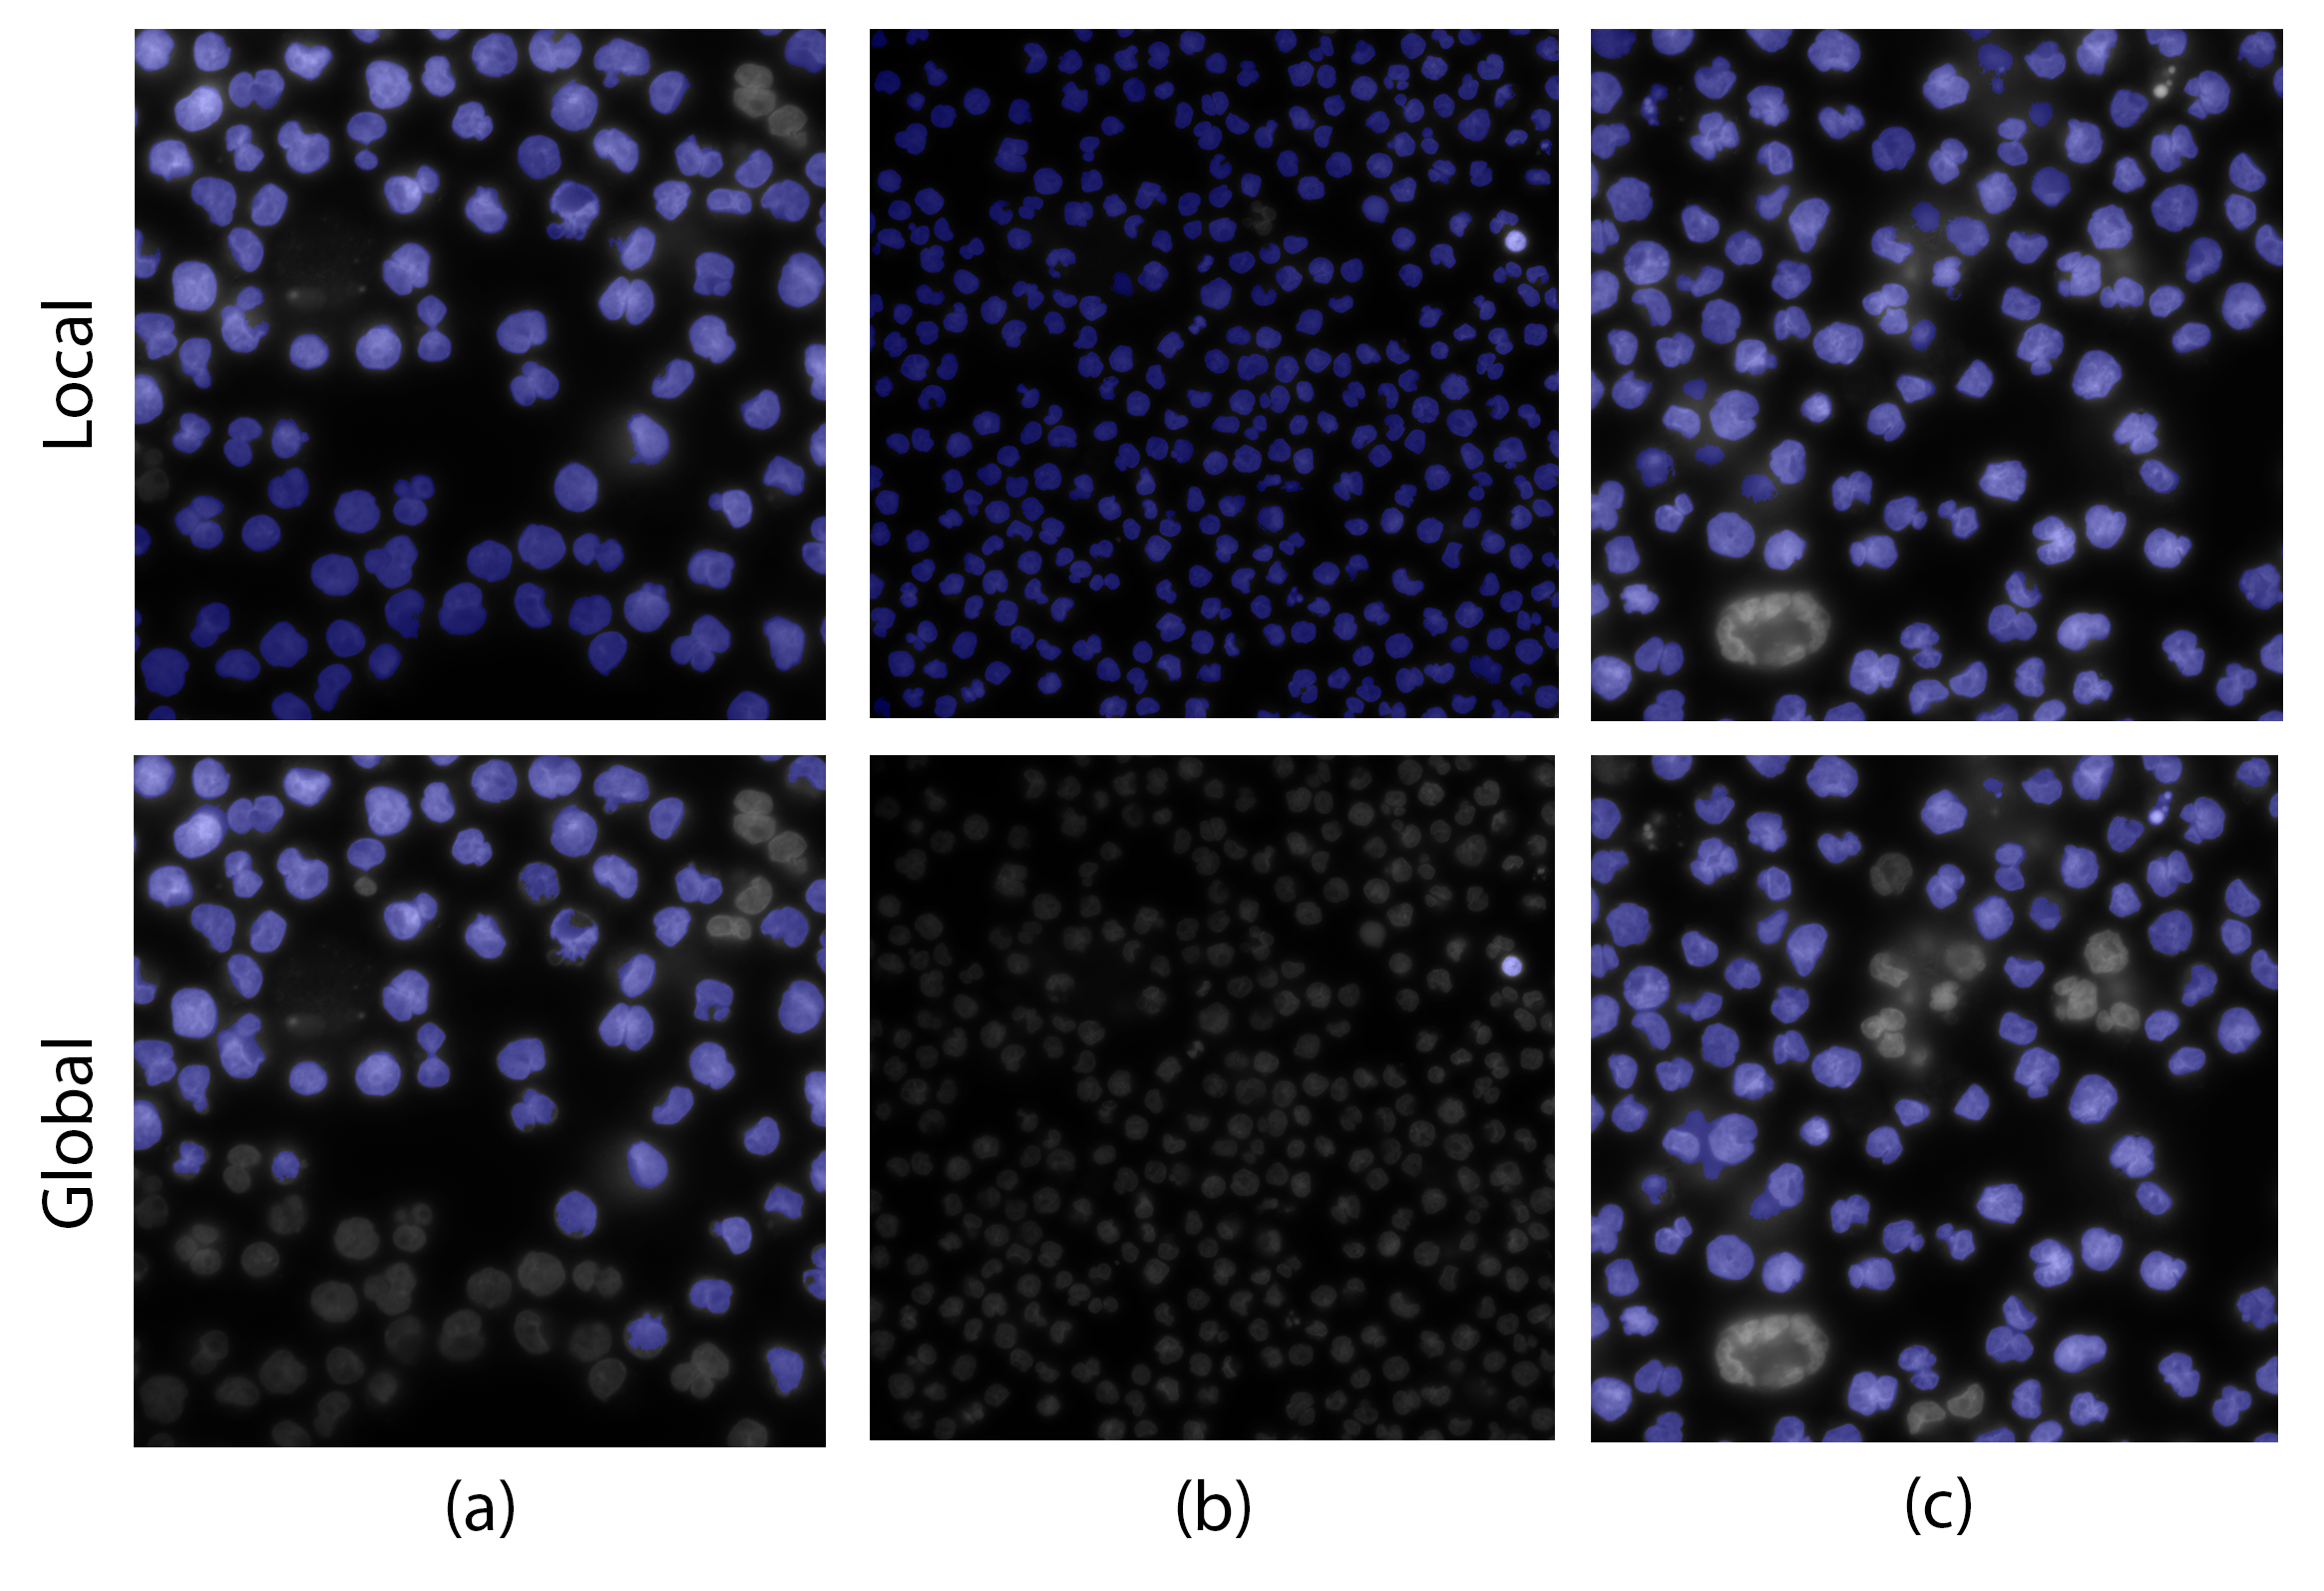
\includegraphics[width=0.6\linewidth]{bilder/difficult-lightning/local-vs-global.png}
		\caption[Local vs. global thresholding]%
        {Local vs. global thresholding. A compasion of the results of local and global thresholding algorithms for three lightning situations in ground truth nuclei fluorescence: (a) --- gradient in image illumination; (b) --- overexposure of one cell resulting in underexposure of all other celss; (c) --- normal conditions. Local thresholding is able to segment foreground (nuclei) much better than a global thresholding approach in all cases.}\label{fig:thresholding-bad-conditions}
	\end{center}
\end{figure}

Although global minumum thresholding method performs better than other approaches it, as any global thresholding algorithm, still has a difficulty in dealing with non-uniform illumination within the images. For visual comparison of global thresholding applied to difficult images see Figure \ref{fig:thresholding-bad-conditions}a, b. Figure \ref{fig:thresholding-bad-conditions}c is an image with equal brightness level, however even there some mistakes do appear.

Therefore for nuclei segmentation a local thresholding algorithm was chosen. With the image size of $2136 \times 2136$, the local neighborhood (or a \textit{block\_ size}) by experimenting with different values was chosen equal to $111$ (\cite{local_thresholding}).

\begin{table}[htb]
    \centering
        \begin{tabular}{||c c||} 
         \hline
         Local Threshold & Global Threshold \\ [0.5ex] 
         \hline\hline
         0.3 sec & 17 sec  \\ 
         \hline
        \end{tabular}
        \caption{Threshold runtime for one image of size $2136 \times 2136$}
        \label{table:threshold-timing}
    \end{table}
    
Of course local thresholding approach has a longer runtime time (see Table \ref{table:threshold-timing}). Therefore when the inference speed is crucial one can still use \textit{global minimum thresholding}. It does performs visually a bit worse that a local threshold (especially for the extreme corrupted cases), however for the normal conditions the performance is quite similar to the local thresholding (Figure \ref{fig:thresholding-bad-conditions}c). As stated in in Algorithm \ref{algorithm:nuclei-segmentation} a local thresholding approach was chosen. One should also keep in mind, that after the model is trained due to its generalization ability the gradient in intensities or overexposure will not be present anymore, as it is related to the image acquisition technique and does not depend on the DIC image itself. For this reason for UNet predictions global minimum thresholding can be successfully used. However, as runtime for not crucial in this case, same postprocessing approach was used for both datasets.